\section{INTEGRABLE FUNCTIONS}
Recall that $o(f,x)$ denotes the oscillation of $f$ at $x$.
\begin{lemma}
    Let $A$ be a closed rectangle and let $f:A\to \F{R}$ be a bounded 
    function such that $o(f, x)<\varepsilon$ for all $x\in A$. Then 
    there is a partition $P$ of $A$ such that $U(f, P)-L(f, P)<\varepsilon\cdot v(A)$.
\end{lemma}

\begin{proof}
    For each $x \in A$ there is a closed rectangle $U_x$,
containing $x$ in its interior, such that $M_{U_x}(f) - M_{U_x}(f) < \varepsilon$.
Since $A$ is compact, a finite number $U_{x_1}, \cdots, U_{x_n}$ of the
sets $U_x$ cover $A$. Let $P$ be a partition for $A$ such that each
subrectangle $S$ of $P$ is contained in some $U_{x_i}$. Then 
$M_s(f) - m_S(f)< \varepsilon$ for each subrectangle $S$ of $P$, so that 
$U(f, P)-L(f, P)=\sum_{S}^{}{M_s(f)-m_S(f)}<\varepsilon\cdot v(A)$.
\end{proof}

\begin{theorem}
    Let $A$ be a closed rectangle and let $f:A\to \F{R}$ a bounded function.
    Let $B=\{x:f\text{ is not continuous at } x\}$. Then $f$ is Integrable if 
    and only if $B$ is a set of measure 0.
\end{theorem}

\begin{proof}
    Suppose first that B has measure 0. Let $\varepsilon > 0$ and
    let $B_\varepsilon = {x: o(f,x) \ge \varepsilon}$. Then $B_\varepsilon \subset B$, 
    so that $B_\varepsilon$ has measure 0. Since (Theorem 1-11) $B_\varepsilon$ is compact, 
    $B_\varepsilon$ has content 0. Thus there is a finite collection $U_1, \cdots, U_n$ of
    closed rectangles, whose interiors cover $B_\varepsilon$, such that $\sum_{i=1}^{n }{v(U_i)}
    <\varepsilon$. Let $P$ be a partition of $A$ such that every subrectangle $S$ of 
    $P$ is in one of two groups (see Figure \ref{Fig 3-1}):
    \begin{figure}[htb]
        \centering
        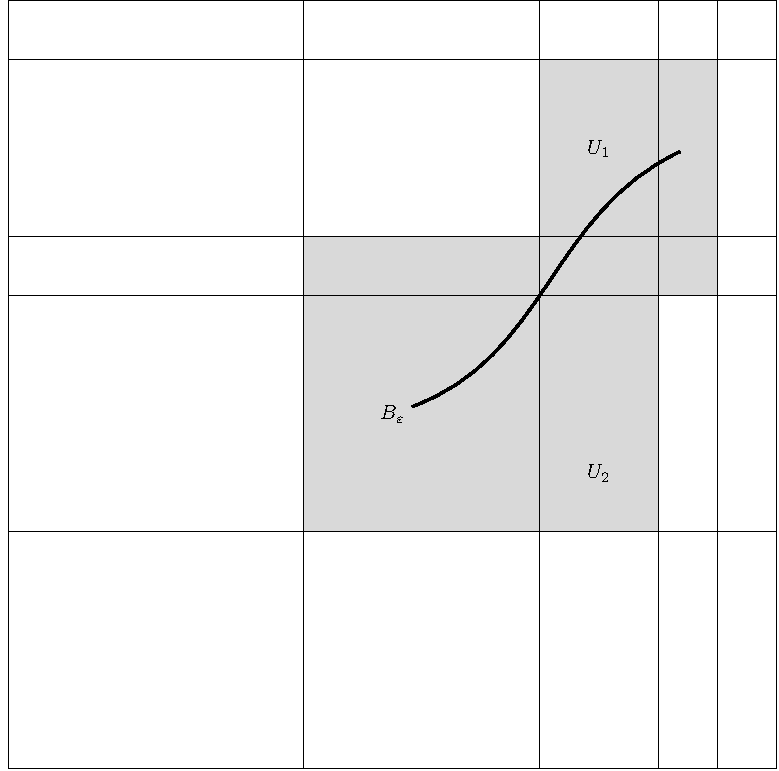
\includegraphics[width=.75\linewidth]{./pics/Fig3-1.pdf}
        \caption{The shaded rectangles are in $\C{S}_1$}
        \label{Fig 3-1}
    \end{figure}

    \begin{enumerate}[label={\upshape(\arabic*)}]
        \item $\C{S}_1$, which consists of subrectangles $S$, such that $S\subset U_i$ for some $i$.
        \item $\C{S}_2$, which consists of subrectangles $S$, with $S\cap B_\varepsilon=\ns$. 
    \end{enumerate}
    Let $|f(x)|<M$ for $x\in A$. Then $M_s(f)-m_S(f)<2M$ for every $S$. Therefore 
    \begin{align*}
        \sum_{S'\subset S_1}^{}{[M_{S'}(f) - m_{S'}(f)]\cdot v(S')} < \varepsilon\cdot v(S)
    \end{align*}

    for $S\in \C{S}_2$. Then 
    \begin{align*}
        U(f, P') - L(f, P')
        & = \sum_{S'\subset S\in \C{S}_1}^{}{[M_{S'}(f) - m_{S'}(f)]\cdot v(S')} \\
        & + \sum_{S'\subset S\in \C{S}_2}^{}{[M_{S'}(f) - m_{S'}(f)]\cdot v(S')} \\
        & < 2M\varepsilon + \sum_{S\in \C{S}_2}^{}{\varepsilon\cdot v(S)}\\
        & \le 2M\varepsilon + \varepsilon\cdot v(A)\\
    \end{align*}

    Since $M$ and $v(A)$ are fixed, this shows that we can find a partition $P'$ with 
    $U(f, P') - L(f, P')$ as small as desired. Thus $f$ is Integrable.

    Suppose, conversely, that $f$ is integrable. Since $B =
    B_1 \cup B_{1/2} \cup B_{1/3} \cup \cdots$, it suffices (Theorem 3-4) to prove
    that each $B_{1/n}$ has measure 0. In fact we will show that each $B_{1/n}$ has 
    content 0 (since $B_{1/n}$ is compact, this is actually equivalent).

    If $\varepsilon>0$, let $P$ be a partition of $A$ such that $U(f, P) - L(f, P) < \varepsilon/n$.
    Let $\C{S}$ be the collection of subrectangles $S$ of $P$ which intersect $B_{1/n}$.
    Then $\C{S}$ is a cover of $B_{1/n}$. Now if $S\in \C{S}$, then $M_S(f)-m_S(f)\ge 1/n$. Thus 
    \begin{align*}
        \frac{1}{n}\cdot \sum_{S\in \C{S}}^{}{v(S)} 
        & \le \sum_{S\in\C{S}}^{}{[M_S(f)-m_S(f)]\cdot v(S)} \\
        & \le \sum_{S}^{}{[M_S(f)-m_S(f)]\cdot v(S)} \\
        & < \frac{\varepsilon}{n}
    \end{align*}
    and consequentlt $\sum_{S\in \C{S}}^{}{v(S)}<\varepsilon$.
\end{proof}

We have thus far dealt only with the integrals of functions
over rectangles. Integrals over other sets\index{Integral!over a set} are easily reduced
to this type. If $C\subset \F{R}$, the \textbf{characteristic function}\index{Function!characteristic}\index{Characteristic function} $\chi_C$ of $C$ is defined by
\begin{align*}
    \chi_C(x) = 
    \left\{\begin{aligned}
        & 0 && x\notin C \\
        & 1 && x\in C
    \end{aligned}\right.
\end{align*}

If $C\subset A$ for some closed rectangle $A$ and $f:A\to \F{R}$ is bounded, then 
$\int_{C }^{}{f}$ is defined as $\int_A f\cdot \chi_C$, provided $f\cdot \chi_C$ is 
Integrable. This certainly occurs (Problem 3-14) if $f$ and $\chi_C$ are Integrable.

\begin{theorem}
    The function $\chi_c: A\to \F{R}$ is integrable if and
    only if the boundary of $C$ has measure 0 (and hence content 0).
\end{theorem}

\begin{proof}
    If $x$ is in the interior of $C$, then there is an open
    rectangle $U$ with $x \in U \subset C$. Thus $\chi_C = 1$ on $U$ and $\chi_C$ is
    clearly continuous at $x$. Similarly, if $x$ is in the exterior of $C$,
    there is an open rectangle $U$ with $X \in U \subset \F{R}^n - C$. Hence
    $\chi_C = 0$ on $U$ and $\chi_C$ is continuous at $x$.
    Finally, if $x$ is in the boundary of $C$, then for every open rectangle $U$ containing
    $x$, there is $y_1 \in U \cap C$, so that $\chi_C(y_1) = 1$ and there is
    $y_2 \in U \cap (\F{R}^n - C)$, so that $\chi_C(y_2) = 0$.
    Hence $\chi_C$ is not continuous at $x$. Thus $\{x: \chi_C \text{ is not continuous at } x\}
    =\text{boundary } C$, and the result follows from Theorem 3-8.
\end{proof}

A bounded set $C$ whose boundary has measure 0 is called
\textbf{Jordan-measurable}\index{Jordan-measurable}. The integral $\int_C1$ is called the ($n$-dimensional) 
\textbf{content}\index{Content} of $C$, or the ($n$-dimensional) \textbf{volume}\index{Volume} of $C$.
Naturally one-dimensional volume is often called \textbf{length}\index{Length}, and two-dimensional 
volume, \textbf{area}. Problem 3-11 shows that even an open set $C$ may not be
Jordan-measurable, so that $\int_Cf$ is not necessarily defined even if $C$ is open 
and $f$ is continuous. This unhappy state of affairs will be rectified soon.


\begin{problems}
    \problem{
        Show that if $f\cdot g:A\to \F{R}$ are integrable, so is $f\cdot g$.
    }
    \problem{
        Show that if $C$ has content 0, then $C \subset A$ for some closed rectangle
        $A$ and $C$ is Jordan-measurable and $\int_A \chi_C = 0$.
    }
    \problem{
        Give an example of a bounded set C of measure 0 such that $\int_A \chi_C = 0$ does not exist.
    }
    \problem{
        If C is a bounded set of measure 0 and $\int_A \chi_c$ exists, show that $\int_A \chi_C = 0$.
        \textit{Hint:} Show that $L(f, P) =0$ for all partitions $P$. Use Problem 3-8.
    }
    \problem{
        If $f:A\to \F{R}$ is non-integrable and $\int_A \chi_C = 0$, show that $\{x:f(x)\neq 0\}$
        has measure 0. \textit{Hint:} Prove that $\{x:f(x)>1/n\}$ has content 0.
    }
    \problem{
        Let $U$ be the open set of Problem 3-11. Show that if $f=\chi_U$ 
        except on a set of measure 0, then $f$ is not integrable on $[0,1]$.
    }
    \problem{
        Show that an increasing function $f: [a,b] \to \F{R}$ is integrable on $[a,b]$.
    }
    \problem{
        If $A$ is a closed rectangle, show that $C \subset A$ is Jordan-measurable
        if and only if for every $\varepsilon > 0$ there is a partition $P$ of $A$ such that
        $\sum_{S\in\C{S}_1}^{}{v(S)} - \sum_{S\in\C{S}_2}^{}{v(S)} <\varepsilon$, where 
        $\C{S}_1$ consists of all subrectangles intersecting $C$ and $\C{S}_2$ all 
        subrectangles contained in $C$.
    }
    \problem[*]{
        If $A$ is a Jordan-measurable set and $\varepsilon > 0$, show that there is a
        compact Jordan-measurable set $C \subset A$ such that $\int_{A-C}1<\varepsilon$.
    }
\end{problems}